\documentclass{llncs}

\usepackage[T1]{fontenc}
\usepackage{algorithmic}
\usepackage{algorithm}
\usepackage{complexity}
\usepackage{times}
\usepackage{graphicx}
\usepackage{multirow}
\usepackage{slashbox}
\usepackage{pstricks,pst-all}



\usepackage{amsmath}
\usepackage{amssymb}
\usepackage{epsfig}
\usepackage{color}


\newcommand{\embnd}{\textit{bnd}}
\newcommand{\cale}{{\cal E}}
\newcommand{\calg}{{\cal G}}
\newcommand{\calp}{{\cal P}}
\newcommand{\calq}{{\cal Q}}
\newcommand{\emlast}{\textit{last}}
\newcommand{\true}{\mbox{\em true}}
\newcommand{\false}{\mbox{\em false}}
\newcommand{\defn}{\stackrel{\mbox{\tiny def}}{=}}
\newcommand{\pfrr}{\Box}
\newcommand{\until}{\textrm{U}} % {\textsf{U}} % \textup{U}\textsc{U}\textmd{U}}
\newcommand{\rmrel}{\textrm{R}} % {\textsf{W}} % \textup{W}\textsc{W}\textmd{W}}
\newcommand{\pevt}{\Diamond}
\newcommand{\nxt}{\bigcirc}
\newcommand{\nnneg}{{\mathbb N}}


\def\qed{\ifmmode\|\else{\unskip\nobreak\hfil
\penalty50\hskip1em\null\nobreak\hfil$\blacksquare$
\parfillskip=0pt\finalhyphendemerits=0\endgraf}\fi}




\newenvironment{list1}{\begin{list}{$\bullet$}
{\topsep 0 pt \parsep 0 pt \partopsep 0 pt \itemsep 0 pt}}{\end{list}}
\newenvironment{list2}{\begin{list}{$-$}
{\topsep 0 pt \parsep 0 pt \partopsep 0 pt \itemsep 0 pt}}{\end{list}}


\begin{document}

\title{Model-Checking Iterated Games%
\thanks{The research was supported
by the National Science Council %(NSF)
grant 97-2221-E-002-129-MY3 and 
by the Engineering and Physical Sciences Research Council %(EPSRC)
grant EP/H046623/1.}}

\author{Chung-Hao Huang$^{1}$ 
\hspace*{5mm} Sven Schewe{$^2$} 
\hspace*{5mm} Farn Wang$^{1,3}$ 
}

\institute{
1: Graduate Institute of Electronic Engineering, National Taiwan University\\
2: Department of Computer Sciences, University of Liverpool\\
3: Department of Electrical Engineering, National Taiwan University \\
}


\maketitle
\thispagestyle{empty}
\pagestyle{plain}
% \baselineskip 18pt

\begin{abstract}
We propose a logic for the definition of the collaborative power of groups of agents to enforce different temporal objectives.
The resulting {\em temporal cooperation logic} ({\em TCL}) extends ATL by allowing for successive definition of strategies for agents and agencies.
Different to previous logics with similar aims, our extension cuts a fine line between extending the power and maintaining a low complexity:
model-checking TCL sentences is EXPTIME complete in the logic, and fixed parameter tractable for specifications of bounded size.
This advancement over non-elementary logics is bought by disallowing 
a too close entanglement between cooperation and competition.
We show how allowing such an entanglement immediately leads to a non-elementary complexity.
%
We have implemented a model-checker for the logic and shown the feasibility of model-checking on a few benchmarks.
\end{abstract}


% \noindent {\bf Keywords:}
% games, turn-based,  
% logic, model-checking, expressiveness


\section{Introduction}


While the verification of traditional linear and 
branching time logics like LTL, CTL, and CTL* \cite{Pnueli77,CE81} 
has been reduced to (repeated) reachability \cite{Holzmann97,KVW00},
the satisfiability checking and synthesis problem has been tightly linked with game theory ever since the seminal works 
of B\"uchi and Landweber \cite{BL69,BL69a}.
With the introduction of {\em alternating time logic} 
({\em ATL}) by Alur, Henzinger, and Kupferman \cite{AHK02} and in automata based $\mu$-calculus model-checking (e.g., \cite{Wilke01}), games have entered into the verification of the correctness of reactive systems.
With game theoretic challenges moving into the focus of researchers who study the specification and design of reactive systems, traditional problems of multi-player games are replacing the former distinction between an adversarial environment and a supportive system.
Instead, we have groups of players that cooperate on some objectives while competing on others.

For particular properties, the intuition that some players represent the system while 
other players represent the environment is, however, still useful.  
Following this intuition, the system wins the game in an execution 
(or a {\em play} in the jargon of game theory) 
if the system specification is fulfilled along it, and it wins the game if it can force a winning play.
System design as a whole for specifications in game logics can rather be compared to designing a game board and to show that the respective group of players (or: agency) has the coalition power required by the system specification.

There are various established game-based specification languages, 
including 
{\em ATL}, {\em ATL}$^*$, the {\em alternating $\mu$-calculus} ({\em AMC}), and 
{\em game logic} ({\em GL}) \cite{AHK02}, 
{\em strategy logics} \cite{CHP10,CLM10,MMV10,MMPV12}, 
{\em coordination logic} \cite{FS10},
{\em stochastic game logic} \cite{BBGK07}, and
{\em basic strategy interaction logic} ({\em BSIL}) \cite{WHY11}
for the specification of the interplay in open systems.  
Each language also comes with a verification algorithm that 
determines whether a winning strategy for the system exists.  
However, there is a gap between the available techniques and the scalability required for industrial applications.
Frankly speaking, none of the languages above represents, in our view, a proper combination of expressiveness for close interaction among agent strategies and efficiency for the verification or refutation of compliance with a specification.
On one hand, logics like ATL, ATL$^*$, AMC, and GL \cite{AHK02} allow 
us to specify the collaborative power of groups of players to enforce a common objective.
This falls short from specifying even the simple properties in 
a typical game.  
For example, it was shown in \cite{WHY11} 
that ATL, ATL$^*$, AMC, and GL \cite{AHK02}  
cannot express that the same strategy of a banking system must allow the clients 
both, to withdraw and to deposit money:
a strategy quantifier in these logics always refers to the strategies of all agents, whereas this property requires to bind first the strategy of the bank, and then refer to different strategies of the clients.
This is arguably a severe restriction when reasoning about real-world problems.  


To solve the expressiveness problem in the above example, 
{\em strategy logics} ({\em SL}) were proposed in \cite{BBGK07,CHP10,MMV10,MMPV12}. 
They allow for the flexible quantification over strategies in logic formulas.  
However, their verification complexity is prohibitively high 
and has inhibited practical application.  

A previous attempt to tame the complexity of strategy interaction \cite{WHY11}, on the other hand, results in a full temporalisation.
This leads to severe restrictions in the entanglement between temporal operators and strategy binding and thus prevents, for example, reasoning about Nash equilibria.

We thus propose to adapt the logic introduced in \cite{WHY11} to 
a new temporal logic called {\em temporal cooperation logic}
({\em TCL}) for this purpose.
%
Let us introduce TCL informally on a game among three prisoners.

\paragraph{\bf Example: Iterated Prisoners' Dilemma.} 
Inspired by the famous prisoners' dilemma, we consider a model where three suspects, who are initially in custody, are interrogated.
In our simplified version, they play in turns (rather than concurrently), and have the choices to either admit or deny the charges made against them.
If all deny, they will be released based on lack of evidence.

However, a suspect may decide to collaborate with the police and betray her peers.
A sole collaborator will be acquitted as a crown witness, while her peers will be sentenced.
But if two or more suspects collaborate with the police, all will be sentenced.

In an iterated prisoners' dilemma, the interplay can continue 
up to an unbounded number of times. 
Such a game is very useful in modelling collaboration and competition 
in networks.  
For example, a strategy in prisoners' dilemma is {\em nice} if 
it does not suggest betrayal initially and only suggests 
betrayal if, in the previous round, another prisoner betrayed 
\cite{Axelrod80}.  
The following TCL sentence states that Prisoner 1 has a nice strategy.
\begin{center} 
\hfill 
$\langle 1\rangle \pfrr ((\langle+\rangle \nxt \neg\mbox{\tt betray}_1)
\vee \bigvee_{a\neq 1}\mbox{\tt betray}_a)$
\hfill (A) 
\end{center} 
$\langle 1\rangle$ is a \emph{strategy quantifier} (SQ), which states
that there exists a strategy of Prisoner 1 to achieve her temporal goal. 
$\langle+\rangle$ is a {\em strategy interaction quantifier} 
({\em SIQ}) %introduced in \cite{WHY11} 
that inherits the strategy from its parent formula. 
Proposition $\mbox{\tt betray}_i$ is an atomic proposition for the betrayal 
of prisoner $i$ at the present state. 
Similarly, we can reflect more involved strategies, such as `Prisoner 2 will always betray when she does not have the power to force Player 1 to always play nice.'
\begin{center} 
\hfill 
$\langle 2\rangle (
(\langle+\rangle \pfrr \mbox{\tt betray}_2) 
\vee \langle+\rangle\pfrr ((\langle+\rangle \nxt \neg\mbox{\tt betray}_1)
\vee \bigvee_{a\neq 1}\mbox{\tt betray}_a))$
\hfill (B) 
\end{center} 

Similar properties can be used to specify {\em forgiving}\footnote{A strategy 
is forgiving if it does not always punish betrayal in the previous round.} 
or other related strategies \cite{Axelrod80}.  
A forgiving strategy of Prisoner 1 
is reflected by the following TCL property. 
\begin{center} 
\hfill 
$\langle 1\rangle \pevt ((\langle+\rangle \nxt \neg\mbox{\tt betray}_1)
\wedge \bigvee_{a\neq 1}\mbox{\tt betray}_a)$
\hfill (C) 
\end{center} 
We can also reason about the existence of Prisoner 2's strategy 
that avoid betrayal if Prisoner 1 can be unforgiving under this strategy. 
\begin{center} 
\hfill 
$\langle 2\rangle (
(\langle+\rangle \pfrr \neg\mbox{\tt betray}_2) 
\vee \langle +1\rangle\pevt ((\langle+\rangle \nxt \neg\mbox{\tt betray}_1)
\wedge \bigvee_{a\neq 1}\mbox{\tt betray}_a))$
\hfill (D) 
\end{center} 
As can be seen, properties like (B) and (D) are relevant in network environments
where plays can be extended round by round
without termination.  
Every agent may track each others' records to decide whether or not to cooperate. 
Such a property cannot be expressed in ATL$^*$, GL, AMC, or BSIL. 
While it can be expressed with SL, the verification complexity of SL is prohibitive.  

In \cite{WHY11}, SIQs can neither override nor revoke strategies assigned by the SQ or SIQs in whose scope they are.
Consequently, BSIL cannot express deterministic Nash equilibria.
To overcome this restriction, we introduce a strategy reset operator that revokes previous strategy assignments.

Let $\mbox{\tt jail}_a$ be a proposition, which states that ``Prisoner $a$ is in jail''.
In TCL,
\begin{center}
\hfill
$\langle 1,2,3\rangle
        \bigwedge_{a\in [1,3]}\big((
        \langle+\emptyset\rangle\pevt \neg \mbox{\tt jail}_a) \vee
        \langle-a\rangle \pfrr \mbox{\tt jail}_a\big)$
\hfill (E)
\end{center}
requires that the tree agents can cooperate such that every agent either eventually leaves prism, or stays for ever in prism regardless of her own strategy under the current strategies of the remaining prisoners.
The SIQ $\langle-a\rangle\psi$ revokes the binding of agent $a$ to her strategy.

% Also in \cite{WHY11}, the universal SIQs $[+A]$ are subject 
% to the restriction that 
% any agent in $A$ may not conflict with an ancestor SQ or SIQ 
% that pass down a strategy with the same agent.   
% As a result, BSIL cannot express the deterministic Nash equilibria. 
% For this purpose, we also presented a strategy reset operator 
% in this work.  
% Let $\mbox{\tt jail}_a$ be the proposition for prisoner $a$ in jail.  
% Specifically, 
% in TCL, the equilibria can be specified with the following property. 
% \begin{center} 
% \hfill 
% $\langle 1,2,3\rangle(
% 	(\bigwedge_{a\in [1,3]}
% 	\langle+\emptyset\rangle\pfrr \mbox{\tt jail}_a)\wedge 
% \bigwedge_{a\in[1,3]}\langle-a\rangle \pfrr\bigwedge_{b\in[1,3];b\neq a}\mbox{\tt jail}_b)$
% \hfill (E) 
% \end{center} 
% SIQ $\langle-a\rangle\psi$ resets the inheritance of any strategy for 
% $a$ declared with the ancestor formulas of $\langle-a\rangle\psi$.  

In this work, we establish that TCL is incomparable with ATL$^*$, GL, and AMC in expressiveness.  
Although the strategy logics proposed in \cite{BBGK07,CHP10,CLM10,MMV10} subsume TCL with their flexible quantification of strategies and binding to strategy variables, 
their model-checking complexities are all doubly exponential time hard.  
In contrast, TCL enjoys an EXPTIME-complete model-checking complexity and fixed parameter tractability when using the length of the formula as parameter, as well as 2EXPTIME completeness of the TCL satisfiability problem for turn-based game graphs.  
TCL thus provides a better balance between expressiveness and complexity / efficiency considerations 
than ATL$^*$, GL \cite{AHK02}, and SL \cite{CHP10,MMV10,MMPV12}.
Given the expressive power as exemplified by the specifications from above, TCL can be viewed as an expressive yet inexpensive subclass of SL \cite{MMV10,MMPV12}.  

\paragraph{\bf Organisation of the Paper.}
Section~\ref{sec.sysmodel} explains turn-based game graphs for the description of multi-agent systems and presents the syntax and semantics of TCL.
Section~\ref{sec.exp} discusses the expressiveness of TCL, establishing that CTL, ATL, LTL, and CTL* can be viewed as syntactic fragments of TCL.
We show that TCL is more expressive than any of these logics while incomparable with ATL$^*$, AMC, and GL \cite{AHK02} in expressiveness, and discuss the effect of a mild extension of TCL. 
In the following sections, we develop an automata based model-checking algorithm and establish the EXPTIME-completeness and 2EXPTIME-completeness of the TCL model-checking and satisfiability problem, respectively.
Finally, we have implement a model-checker and validated the feasibility of using TCL on a set of benchmarks.


\section{System Models and TCL \label{sec.sysmodel}}

\subsection{Turn-based game graphs \label{subsec.tb.gg}} 

A {\em turn-based} game is played by a finite number $m$ of agents, indexed $1$ through $m$.
A game is a tuple $\calg=\langle m,\calq,r,\omega,P,\lambda,E\rangle$, where
\begin{list1}
\item 
	Parameter $m$ is the number of agents in the game.
\item 
	$\calq$ is the set of states and
% \item 
	$r\in \calq$ is the {\em initial state} (or root) of $\calg$.
\item 
	$\omega:\calq\mapsto [1,m]$ is a function that specifies the
    owner of each state.
    Only the owner of a state makes choices at the state.
\item 
	$P$ is a finite set of atomic propositions.
\item 
	$\lambda:\calq\mapsto 2^P$ is a proposition labelling function.
\item 
	$E\subseteq \calq \times \calq$ is the set of transitions.
\end{list1}
For ease of notation, we denote with 
$\calq_a = \{q \in \calq \mid \omega(q)=a\}$ 
the states owned by an agent $a$.

In Figure~\ref{fig.gg.mem.fin}, we have the graphical representation of 
a turn-based game graph.  
\begin{figure}[t]
\begin{center}
\begin{picture}(0,0)%
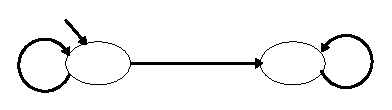
\includegraphics{gg.mem.fin60.eps}%
\end{picture}%
\setlength{\unitlength}{4144sp}%
%
\begingroup\makeatletter\ifx\SetFigFont\undefined%
\gdef\SetFigFont#1#2#3#4#5{%
  \reset@font\fontsize{#1}{#2pt}%
  \fontfamily{#3}\fontseries{#4}\fontshape{#5}%
  \selectfont}%
\fi\endgroup%
\begin{picture}(3310,861)(-169,-285)
\put(2490,-39){\makebox(0,0)[lb]{\smash{{\SetFigFont{7}{8.4}{\rmdefault}{\mddefault}{\updefault}{\color[rgb]{0,0,0}$w'$}%
}}}}
\put(2437,-171){\makebox(0,0)[lb]{\smash{{\SetFigFont{7}{8.4}{\rmdefault}{\mddefault}{\updefault}{\color[rgb]{0,0,0}$\{q\}$}%
}}}}
\put(376,-39){\makebox(0,0)[lb]{\smash{{\SetFigFont{7}{8.4}{\rmdefault}{\mddefault}{\updefault}{\color[rgb]{0,0,0}$u'$}%
}}}}
\put(350,-171){\makebox(0,0)[lb]{\smash{{\SetFigFont{7}{8.4}{\rmdefault}{\mddefault}{\updefault}{\color[rgb]{0,0,0}$\{p\}$}%
}}}}
\put(1090,-171){\makebox(0,0)[lb]{\smash{{\SetFigFont{7}{8.4}{\rmdefault}{\mddefault}{\updefault}{\color[rgb]{0,0,0}$\emptyset$}%
}}}}
\put(1777,-39){\makebox(0,0)[lb]{\smash{{\SetFigFont{7}{8.4}{\rmdefault}{\mddefault}{\updefault}{\color[rgb]{0,0,0}$w$}%
}}}}
\put(1803,-171){\makebox(0,0)[lb]{\smash{{\SetFigFont{7}{8.4}{\rmdefault}{\mddefault}{\updefault}{\color[rgb]{0,0,0}$\emptyset$}%
}}}}
\put(1433,463){\makebox(0,0)[lb]{\smash{{\SetFigFont{7}{8.4}{\rmdefault}{\mddefault}{\updefault}{\color[rgb]{0,0,0}$v$}%
}}}}
\put(1433,331){\makebox(0,0)[lb]{\smash{{\SetFigFont{7}{8.4}{\rmdefault}{\mddefault}{\updefault}{\color[rgb]{0,0,0}$\emptyset$}%
}}}}
\put(1063,-39){\makebox(0,0)[lb]{\smash{{\SetFigFont{7}{8.4}{\rmdefault}{\mddefault}{\updefault}{\color[rgb]{0,0,0}$u$}%
}}}}
\end{picture}%
\\
$\nxt$ belongs to Agent 1 and $\pfrr$ belongs to Agent 2.
\end{center}
\caption{A turn-based game graph}
\label{fig.gg.mem.fin}
\end{figure} 
The ovals and squares represent states while the arcs represent 
state transitions.  
We also put down the $\lambda$ values inside the corresponding states.  

For convenience, in the remaining part of the 
manuscript, we assume that we are always in the context 
of a given game graph
$\calg=\langle m,\calq,r,\omega,\calp,\lambda,\cale\rangle$.
Thus, when we write $\calq,r,\omega,\calp,\lambda$, and $\cale$, 
we respectively refer to the components $\calq$, $r$, 
$\omega$, $P$, $\lambda$, and $E$ of this $\calg$.  

% A state predicate of $\calp$ is a Boolean combination of elements in $\calp$.
% We let $\emstp(\calp)$ be the set of state predicates of $\calp$.
% The satisfaction of a state predicate $\eta$ at a state $q$,
% in symbols $q\models \eta$, is defined in a standard way.
% \begin{list1} 
% \item $q\models p$ if and only if $p\in\lambda(q)$.  
% \item $q\models\neg \eta$ if and only if $q\not\models \eta$. 
% \item $q\models \eta_1\vee\eta_2$ if and only if $q\models \eta_1$ or 
%   $q\models\eta_2$.  
% \end{list1} 

A {\em play} $\rho$ is an infinite path $q_0 q_1\ldots$ in $\calg$ 
such that, for every $k\in \nnneg$, 
$(q_k,q_{k+1})\in \cale$.  
$\rho$ is {\em initial} if $q_0=r$. 
For every $k\geq 0$, we let $\rho(k)$ denote $q_k$.
Also, given $h\leq k$,
we let $\rho[h,k]$ denote $\rho(h)\ldots\rho(k)$ and
$\rho[h,\infty)$ denote the infinite tail of $\rho$
from $\rho(h)$. 

A {\em play prefix} is a finite segment of a play from the beginning of
the play.  
Given a play prefix $\pi=q_0q_1\ldots q_n$, 
$|\pi|=n+1$ denotes the length of the prefix.
Given a $k\in [0,|\pi|-1]$, we let $\pi(k)=q_k$.  
For convenience, we use $\emlast(\pi)$ to denote the 
last state in $\pi$, i.e., $\pi(|\pi|-1)$.  

For an agent $a\in [1,m]$,
a {\em strategy} $\sigma$ for $a$ is
a function from $\calq^*\calq_a$ to $\calq$ such that
for every $\pi\in \calq^*\calq_a$,
$\sigma(\pi)\in \calq$ with $\big(\emlast(\pi),\sigma(\pi)\big)\in \cale$.

An {\em agency} $A$ of $[1,m]$ is a subset of $[1,m]$.
In a short hand notation, we often drop the curly brackets in the set notation, in particular for singleton and empty sets.
For example, ``$1,3,4$'' is a short hand for $\{1,3,4\}$.

A play $\rho$ is \emph{compatible} with a strategy $\sigma_a$ of an agent $a\in [1,m]$ iff, for every $k\in \mathbb N$, $\omega(\rho(k))=a$ implies $\rho(k+1)=\sigma(\rho[0..k])$.




\subsection{TCL Syntax \label{subsec.bsil.syntax}}


A TCL formula $\phi$ is constructed with the following three syntax rules.
\smallskip

\noindent
% \begin{center}
$\begin{array}{rcl}
\phi    & ::= & p\;|\; \neg\phi_1 \;|\; \phi_1\vee \phi_2
    \;|\; \langle  A\rangle \psi
    \\
\psi  & ::= & \phi \;|\; \eta \;|\; \psi_1\vee \psi_2\;|\; \psi_1\wedge \psi_2
    \;|\; \langle+A\rangle \psi_1
    \;|\; \langle+A\rangle\nxt\psi_1 
    \;|\; \langle+A\rangle\eta_1\until \psi_1
    \;|\; \langle+A\rangle\psi_1\rmrel \eta_1 \\
    & | & \langle-A\rangle \psi_1
    \;|\; \langle-A\rangle\nxt\psi_1 
    \;|\; \langle-A\rangle\eta_1\until \psi_1
    \;|\; \langle-A\rangle\psi_1\rmrel \eta_1 
    \\
\eta  & ::= & \phi \;|\; \eta_1\vee \eta_2\;|\; \eta_1\wedge \eta_2
    \;|\; \langle+\rangle\nxt\eta_1 
    \;|\; \langle+\rangle\eta_1\until \eta_2
    \;|\; \langle+\rangle\eta_1\rmrel \eta_2 \\
    & | & \langle-A\rangle\nxt\eta_1 
    \;|\; \langle-A\rangle\eta_1\until \eta_2
    \;|\; \langle-A\rangle\eta_1\rmrel \eta_2 
\end{array}$
% \end{center}
\smallskip

Here, $p$ is an atomic proposition in $\calp$ and $A\subseteq \{1,\ldots,m\}$ is an agency.  
Property $\langle A\rangle\psi_1$ is an (existential) 
strategy quantification (SQ) specifying that
there exist strategies of the agents in $A$
that make all plays consistent with these strategies satisfy $\psi_1$.
Property $\langle+A\rangle\psi_1$ is an (existential) 
strategy interaction quantification (SIQ) and 
can only occur bound by an SQ.
Intuitively, $\langle+A\rangle\psi_1$ means that there exist strategies of the agents in $A$
that work with the strategies introduced by the ancestor formulas.
Likewise, $\langle -A \rangle$ indicates a revocation of the strategy binding for the agents in $A$.
$\langle + \rangle$ is an abbreviation for $\langle + \emptyset\rangle$ or, equivalently $\langle - \emptyset \rangle$.
Thus, it neither binds nor revokes the binding of the strategy of any agent.
Yet, it provides a temporalisation in that it provides a tree formula that can be interpreted at a particular point.

% For convenience, we call an SQ also as an SIQ that interacts with 
% no ancestor formula strategies. 

`$\until$' is the {\em until} operator.  
The property $\psi_1\until\psi_2$ specifies a play along which 
$\psi_1$ is true until $\psi_2$ becomes true.  
Moreover, along the play, $\psi_2$ must eventually be fulfilled.   
`$\rmrel$' is the {\em release} operator.  
Property $\psi_1\rmrel\psi_2$ specifies a play along which either 
$\psi_2$ is always true or $\psi_2\until(\psi_1\wedge\psi_2)$ 
is satisfied. (Release is dual to until: $\neg(\phi_1 \until \phi_2) \, \Leftrightarrow \, \neg \phi_2 \rmrel \neg \phi_1$.)

In the following we may use $\langle?A\rangle\psi$ to conveniently 
denote an SQ or SIQ formula with `$?$' is empty, `+', or `-'.  
An SIQ $\langle\pm A\rangle\psi$ is called non-trivial if 
$A$ is not empty, and trivial otherwise. 

Formulas $\phi$ are called {\em TCL} {\em formulas}, {\em sentences}, or 
{\em state formulas}.  
Formulas $\psi$ and $\eta$ are called {\em tree formulas}.  
Note that we strictly require that non-trivial strategy interaction cannot 
cross path modal operators.  
This restriction is important because it offers a sufficient level of locality to efficiently model-check a system against a TCL property.
To illustrate this and to provide a simple extension that offers more expressive power to the cost of a much higher complexity, we informally discuss a small extension,
\emph{extended TCL} (ETCL), where the production rule of $\psi$ also contains $\neg \psi$ and show that it can be used to encode ATL$^*$, and the realisability problem of prenex QPTL can be reduced to ETCL model-checking.

%  and allows us to analyse the interaction 
% of strategies locally in a state and 
% then enforce the interaction along all paths from the state.  


For convenience, we also have the following shorthand notations.
\begin{center}
$\begin{array}{rclcrcl}
\true
& \equiv & p\vee(\neg p) 
& \hspace*{10mm} & % \\
\false
& \equiv & \neg\true \\
\phi_1\wedge \phi_2
& \equiv & \neg((\neg\phi_1)\vee(\neg\phi_2)) 
& \hspace*{10mm} & % \\
\phi_1\Rightarrow \phi_2
& \equiv & (\neg \phi_1)\vee \phi_2 \\
\pevt \phi_1
& \equiv & \true\,\until \phi_1 
& \hspace*{10mm} & % \\
\pfrr \phi_1
& \equiv & \false\,\rmrel \phi_1 \\
% \neg\psi_1\until\psi_2
% & \equiv & \psi_1\rmrel \psi_2 
% & \hspace*{10mm} & % \\
% \neg\psi_1\rmrel\psi_2
% & \equiv & \psi_1\until \psi_2 \\
\neg\nxt \phi_1
& \equiv & \nxt\neg\phi_1 
& \hspace*{10mm} & % \\
\; \langle A\rangle \nxt\psi_1 
& \equiv & \langle A\rangle \langle+\rangle\nxt\psi_1 \\
\; \langle A\rangle \psi_1\until\psi_2
& \equiv & \langle A\rangle\langle+\rangle \psi_1\until\psi_2 
& \hspace*{10mm} & % \\
\; \langle A\rangle \psi_1\rmrel\psi_2  
& \equiv & \langle A\rangle \langle+\rangle\psi_1 \rmrel\psi_2 \\
% & \hspace*{10mm} & % \\
% \; \langle A\rangle \psi_1\until\psi_2
% & \equiv & \langle A\rangle\langle+\rangle \psi_1\until\psi_2 \\
\end{array}
$
\end{center} 
In general, it would also be nice to have the universal SQs and 
SIQs as duals of existential SQs and SIQs, respectively. 
Couldn't we add, or encode by pushing negations to state formulas, 
a property of the form $[+A]\psi_1$, meaning that, for all strategies of agency $A$,  $\psi_1$ will be fulfilled? 
In principle, this is indeed no problem, and extending the semantics would be simple.
This logic would be equivalent to allowing for negations in the production rule of $\psi$.
The problem with this logic is that it is too succinct.
We will briefly discuss in the following section that model-checking becomes non-elementary if we allow for such negations.

% Note, however, that an introduction of negations in the production rule of $\eta$ is only notational sugar.
% As the SIQs in the $\eta$ production rule do not introduce strategies, they are self-dual, and negations can be pushed inside.
% (Cf.\ example (E) from the introduction, where the left hand side of implication can be replaced by
% $( \langle+\emptyset\rangle\pevt \neg \mbox{\tt jail}_a)
% \vee \langle-a\rangle \pfrr \mbox{\tt jail}_a$.)

% All TCL formulas are {\em well-formed} 
% since all their SIQs occur inside
% an SQ beginning with $\langle  A\rangle$
% for some $A$.

From now on, we assume that we are always in the context of a
given TCL sentence. % $\chi$.  






\subsection{TCL Semantics 
  \label{subsec.psil.semantics}}

In order to prepare the definition of a semantics for TCL formulas, 
we start with the definition of a semantics for sentences 
of the form $\langle A \rangle \psi$, where $\psi$ does not contain any SQs.
We call these formulas \emph{primitive} TCL formulas.

Due to the design of TCL, strategy bindings can only effectively happen at non-trivial SQs $\langle A \rangle$ and 
when a non-trivial SIQ $\langle +B\rangle$ is interpreted.
% Moreover, for a subformula $\psi_1\until\psi_2$ 
% (or $\psi_1\rmrel\psi_2$), there is no new strategy binding in 
% $\psi$ to interact with those bound to $\psi_1\until\psi_2$ 
% (or $\psi_1\rmrel\psi_2$).  
%
To ease referring to these strategies, we first define the \emph{bound agency} of a subformulas $\phi$ of a TCL sentence $\chi$, denoted $\embnd(\phi)$, as follows.
\begin{list1} 
\item For state formulas $\phi$, $\embnd(\phi)= \emptyset$.  
\item For state formulas $\langle A \rangle \psi$,  $\embnd(\psi)= A$ (unless $\psi$ is a state formula).
\item For tree formulas $\psi_1=\langle +A \rangle \psi_2$,  $\embnd(\psi_2) = \embnd(\psi_1) \cup A$.
\item For tree formulas $\psi_1=\langle -A \rangle \psi_2$,  $\embnd(\psi_2) = \embnd(\psi_1) \smallsetminus A$.
\item For all other tree formulas $\psi_1$ or $\psi_2$ with $\psi = \psi_1 \mathsf{OP} \psi_2$, with $\mathsf{OP} \in \{\wedge,\vee,\mathcal U, \mathcal R\}$, we have $\embnd(\psi_1) = \embnd(\psi)$ or $\embnd(\psi_2) = \embnd(\psi)$, respectively.
\end{list1} 
$\embnd$ shows, which agents have strategies assigned to them 
by an SIQ or SQ.
Note that this leaves the $\embnd$ undefined for all state formulas not in the scope of an SQ formulas.
For completeness, we could define $\embnd$ as empty in these cases, but a definition will not be required in the definition of the semantics.

As the introduction of additional strategies through non-trivial SIQ $\langle +B\rangle$ is governed by a \emph{positive} 
Boolean combination, all strategy selections can be performed concurrently.
Such a design leads us to the concept of strategy schemes.

A {\em strategy scheme} $\sigma$ is the set of strategies introduced by any non-trivial SQ $\langle A \rangle$ or SIQ $\langle + A \rangle$.
By abuse of notation, we use $\sigma[\phi,a]$ to identify such a strategy.
Read in this way, $\sigma$ can be viewed as a partial function from subformulas and their bound agencies to strategies.
Thus, $\sigma[\phi,a]$ is defined if $a\in \embnd(\phi)$ is in the bound agency of $\phi$.

% The SIQ or SQ operator introducing a strategy for $a$ can be found by walking up the formula tree, starting at $\phi$, and stopping once a formula $\psi$ starting with $\langle A \rangle$ or $\langle + A \rangle$ with $a\in A$ is hit.
% $\sigma[\phi,a]$ refers to the strategy for Agent $a$ introduced by this quantifier.

For example, given a strategy scheme $\sigma$ for a 
TCL sentence $\langle 1\rangle \pevt ((\langle+2\rangle \nxt p)\wedge\langle 2\rangle\pfrr q)$, 
the strategy used in $\sigma$ by Agent $1$ to enforce 
the whole formula can be referred to by
\[\sigma[\langle 1\rangle \pevt ((\langle+2\rangle \nxt p)\wedge\langle 2\rangle\pfrr q),1],\]
but also by $\sigma[\langle+2\rangle \nxt p,1]$, while $\sigma[\langle 2\rangle\pfrr q,1]$ is undefined.
% the one to enforce $\langle+2\rangle \nxt p$ by Agent $2$ is 
% named $\sigma[\langle+2\rangle \nxt p,2]$.  


We use a simple tree semantics for TCL formulas. 
A (computation) tree $T_r$ is obtained by unravelling $\calg$ from $r$  
and expand the ownership 
and labelling functions from $\calg$ to $T_r$ in the natural way.
Technically, we have the following definition.  

\paragraph{\bf Definition: Computation Tree.} 
A {\em computation tree} for a turn based game $\calg$ from a state $q$, 
denoted $T_q$, is the smallest set of play prefixes that contains $q$ and, for all $\pi\in T$ and $(\emlast(\pi),q')\in \cale$, $\pi q'\in T$.
\qed 


The {\em strategy-pruned} tree for a tree node $\pi$, 
a strategy scheme $\sigma$,
and a subformula $\psi_1$ of $\chi$ from a state $q$, 
in symbols $T_q\langle\pi,\sigma,\psi_1\rangle$, 
is the smallest subset of $T_q$ such that: 
\begin{list1} 
\item $\pi\in T_q\langle\pi,\sigma,\psi_1\rangle$;  
\item for all $\pi' \in T_q\langle\pi,\sigma,\psi_1\rangle$ 
  with $\omega\big((\emlast(\pi')\big)\notin\embnd(\psi_1)$ 
  and $(\emlast(\pi'),q')\in \cale$, 
  $\pi' q'\in T_q\langle\pi,\sigma,\psi_1\rangle$;  
\item for all $\pi' \in T_q\langle\pi,\sigma,\psi_1\rangle$,  
  $a=\omega\big((\emlast(\pi')\big)$, and 
  $q'=\sigma[\psi_1,a](\pi')$ 
  with $a\in\embnd(\psi_1)$, 
%   $(\emlast(\pi),q') \in \cale$ and 
  $\pi' q' \in T_q\langle\pi,\sigma,\psi_1\rangle$.
\end{list1}
Given a computation tree or a strategy-pruned tree $T$ and a node $\pi\in T$, 
for every $\pi q\in T$, we say that $\pi q$ is a successor of $\pi$ in $T$. 
A play $\rho$ is a \emph{limit of $T$} (or an infinite path in $T$), in symbols $\rho\stackrel{\infty}\in T$, 
if there are infinitely many prefixes of $\rho$ in $T$. 


We now define the semantics of subformulas of primitive TCL formulas 
inductively as follows.  
% We introduce the semantics of TCL formulas inductively, 
% based on atomic propositions, Boolean combinations, and 
% semantics for primitive TCL formulas, 
% where a state formula is \emph{primitive} 
% iff it has the form $\langle A \rangle \psi$ 
% while none of its true subformulas has this form.
Given the computation tree $T_q$ of $\calg$, a tree node $\pi\in T_q$, 
and a strategy scheme $\sigma$, 
we write $T_q,\pi,\sigma\models\psi_1$ to denote that 
$T_q$ satisfies $\psi_1$ at node $\pi$ with strategy scheme $\sigma$.

While the notation might seem heavy on first glance, note that the truth for state formulas merely depends on the state $\emlast(\pi)$ in which they are interpreted, and the tree formulas are simply interpreted on a strategy pruned tree rooted in $\pi$ and defined by the strategy scheme.
\begin{list1}
\item For state formulas $\phi$ other than SQ formulas,
  we use the state formula semantics:
$T_q,\pi,\sigma\models \phi$ iff $\calg,\emlast(\pi) \models \phi$, 
with the usual definition.  
\begin{list2}
\item  $\calg,q \models p$ if, and only if, $p\in\lambda(q)$,
\item  $\calg,q \models \neg \phi$ if, and only if, $\calg,q \not\models \phi$,
\item  $\calg,q \models \phi_1 \vee \phi_2$ if, and only if, $\calg,q \models \phi_1$ or $\calg,q \models \phi_2$, and
\item  $\calg,q \models \phi_1 \wedge \phi_2$ if, and only if, $\calg,q \models \phi_1$ and $\calg,q \models \phi_2$.
\end{list2}
(Note that this allows for using negation for state formulas.)

\item $T_q,\pi,\sigma \models \psi_1\vee\psi_2$ iff
    $T_q,\pi,\sigma \models \psi_1$
    or $T_q,\pi,\sigma \models \psi_2$.
     \mbox{(The $\psi_i$ are no state formulas.)}
\item $T_q,\pi,\sigma\models \psi_1\wedge\psi_2$ iff
    $T_q,\pi,\sigma\models \psi_1$
    and $T_q,\pi,\sigma\models \psi_2$ hold.
    
\item $T_q,\pi,\sigma\models \langle \pm A \rangle \nxt \psi$ iff,
     for all successors $\pi q'$ of $\pi$ 
     in $T_q\langle \pi,\sigma,\langle \pm A \rangle\nxt\psi_1\rangle$, 
     $T_q,\pi q',\sigma \models \psi$ holds.  
    
\item $T_q,\pi,\sigma \models \langle \pm A \rangle \psi_1\until\psi_2$ iff, for all limits 
    $\rho\stackrel{\infty}\in T_q\langle \pi,\sigma, \langle \pm A \rangle\psi_1\until\psi_2\rangle$, 
    there is a $k \geq |\pi|-1$ 
    such that $T_q,\rho[0,k],\sigma \models \psi_2$ and, 
    for all $h\in [|\pi|-1,k-1]$, 
    $T_q,\rho[0,h],\sigma\models \psi_1$ hold. 
\item $T_q,\pi,\sigma \models \langle \pm A \rangle \psi_1\rmrel\psi_2$ iff, 
    for all limits 
    $\rho\stackrel{\infty}\in T_q\langle\pi,\sigma,\langle \pm A \rangle\psi_1\rmrel\psi_2\rangle$, one of the following two restrictions 
    are satisfied. 
    \begin{list2} 
    \item For all $k \geq |\pi|-1$, $T_q,\rho[0,k],\sigma \models \psi_2$. 
    \item There is a $k\geq |\pi|-1$ such that 
      $T_q,\rho[0,k],\sigma\models \psi_1\wedge\psi_2$, and, 
      for all $h\in [|\pi|-1,k]$, $T_q,\rho[0,h],\sigma\models \psi_2$.
    \end{list2} 
\item $T_q,\pi,\sigma\models \langle \pm A \rangle \psi_1$ iff
    $T_q,\pi,\sigma \models \psi_1$.
\item $\calg, q \models \langle A \rangle \psi_1$ iff there is a strategy scheme $\sigma$ such that
    $T_q,q,\sigma \models \psi_1$.
\end{list1}

If $\phi_1$ is a TCL sentence %and $T_q,q,\sigma\models\phi_1$ 
% for some strategy scheme $\sigma$,
% then we may simply write $\calg,q\models\phi_1$.  
% If
then we write $\calg\models\phi_1$ for $\calg,r\models\phi_1$.


Note that, while asking for the existence of a strategy scheme refers to all strategies introduced by some SQ or SIQ in the TCL sentence, only the strategies introduced by the respective SQ and the SIQs in its scope are relevant.

The simplicity of the semantics is owed to the fact that 
it suffices to introduce new strategies at the points 
where eventualities become true for the first time.
Thus, they do not really depend on the position 
in which they are invoked and we can guess them up-front. 
(Or, similarly, together with the points on the unravelling 
where they are invoked.)
%
This is possible, simply because the validity of state formulas (and hence of TCL sentences) cannot depend on the validity of the left hand side of an until (or the right hand side of a release) \emph{after} the first time it has been satisfied. 






\section{Expressiveness of TCL \label{sec.exp}}

Note that TCL is not a superclass of BSIL since 
BSIL allows for negation in front of SIQs while TCL does not. 
However, by examining the proofs in \cite{WHY11} 
for the inexpressibility of BSIL properties by ATL$^*$, GL, and AMC, 
we find that the BSIL sentence used in the proofs is also a TCL sentence. 
This leads to the conclusion that 
there are properties expressible in TCL but cannot 
be expressed in ATL$^*$, GL, and AMC.  

{\lemma \label{lemma.express.incomp1} 
There are TCL sentences that cannot be expressed 
in any of ATL$^*$, GL, or AMC.  
} 
\qed 


TCL is, in fact, not only a powerful logic, 
but also contains important logics either as syntactical fragments or can embed them in a straight forward way.
ATL and CTL can be viewed as syntactic fragments of TCL.

But it is also simple to embed LTL and even CTL$^*$.
We start with $\exists$LTL, the less used variant 
where one is content if one path satisfies the formula.
% Let $A$ denote the set of all agents.
We then translate an LTL formula, which we assume w.l.o.g.\ 
to be in negative normal form 
(negations only in front of atomic propositions).
Then ``there is a path that satisfies $\phi$'' is equivalent to
$\langle 1,\ldots,m \rangle \widehat{\phi}$, where $\widehat{\phi}$ is derived from $\phi$ by replacing every occurrence of $\nxt$, $\until$, and $\rmrel$ by
$\langle + \rangle \nxt$, $\langle + \rangle \until$, and $\langle + \rangle \rmrel$, respectively.
%
The simple translation is possible because the formula $\widehat{\psi}$ 
is de-facto interpreted over a path, 
the path formed by the joint strategy of the agency $[1,m]$.
The $\langle + \rangle$ operators we have added have no effect on the semantics in such a case, just as a CTL formula can be interpreted as the LTL formula obtained by deleting all path quantifiers when interpreted over a word.

Consequently, we have the expected semantics for $\forall LTL$:  ``all paths satisfy $\phi$'' is equivalent to
$\neg \langle A \rangle \widehat{\neg\phi}$, where $\neg \phi$ is assumed to be re-written in negative normal form.
% This immediately implies that TCL model-checking is PSPACE hard.
% 
The encoding of $\exists$LTL and $\forall$LTL can easily be extended to the encoding of CTL$^*$.  
%
{\lemma \label{lemma.express.ctl.star}
TCL is more expressive than CTL$^*$ and LTL.  
}
\qed 

This encoding does not extend to ATL$^*$.
$\langle 1\rangle ((\pfrr p)\vee \pfrr q)$  is an ATL$^*$ property that cannot be 
expressed with TCL.

This is different from the 
% \begin{center} 
ATL property $(\langle 1\rangle \pfrr p)\vee \langle 1\rangle\pfrr q$ 
% \end{center} 
or the
% \begin{center} 
TCL property
\mbox{$\langle 1\rangle ((\langle+\rangle\pfrr p)\vee \langle +\rangle\pfrr q)$}. 
% \end{center} 
In fact, the proofs and examples in \cite{WHY11} 
can also be applied in this work to show that 
there are properties of ATL$^*$ (or GL, or AMC) 
that cannot be expressed with TCL.  
This leads to the following lemma. 

{\lemma \label{lemma.express.incomp2} 
TCL is incomparable in expressiveness with ATL$^*$, GL, and AMC.  
} 
\qed 

Note, however, that allowing for a negation in the definition of $\psi$ would change the situation.
Then an ATL$^*$ formula $\langle A \rangle \psi$ 
(assuming for the sake of simplicity that $\psi$ is an LTL formula), 
would become
$\langle A \rangle \neg \langle + [1,m] \smallsetminus A \rangle \widehat{\neg \psi}$ in the extended version of TCL.
The translation extends to full ATL$^*$, but this example also demonstrates why negation is banned: even without nesting, we can, by encoding ATL$^*$, encode a 2EXPTIME complete model-checking problem, losing the appealing tractability of our logic.

In fact, it is easy to reduce the realisability problem of prenex QPTL, and hence a non-elementary problem, to the model-checking problem of extended TCL.
Using the game structure from Figure \ref{fig.nonelementary}, we can encode the realisability of a prenex QPTL formula with $n-1$ variables, for simplicity of the form
$\forall p_2 \exists p_3 \forall p_4 \ldots \exists p_n \phi$, where $p_2,\ldots,p_n$ are all propositions occurring in $\phi$.
We reduce this to model-checking the formula 
\[\phi'=\langle 1 \rangle \neg \langle +2 \rangle \neg \langle +3 \rangle \neg \langle +4 \rangle \neg \ldots \neg \langle +n \rangle (\psi_\phi \wedge \langle + \rangle \pfrr p_1),\]
where $\psi_\phi$ can be obtained from $\widehat{\phi}$ by replacing
\begin{list1}
\item every literal $p_i$ by $\langle - 1 \rangle \langle + 1 \rangle \nxt (p_i \wedge \langle + \rangle \nxt p_i)$, and
\item every literal $\neg p_i$ by $\langle - 1 \rangle \langle + 1 \rangle \nxt (p_i \wedge \langle + \rangle \nxt \neg p_i)$.
\end{list1}

These formulas are technically not extended TCL formulas as $\langle +i \rangle \psi_1$ is not part of the production rule of $\psi$,  but $\langle +i \rangle \psi_1$ can be used as an abbreviation for $\langle +i \rangle \false \until \psi_1$.

Checking satisfiability of $\phi$ is is equivalent to model-checking $\phi'$ on the game shown in Figure \ref{fig.nonelementary}. 
The game has $n+1$ nodes, agents, and atomic propositions.
The nodes in Figure \ref{fig.nonelementary} are labeled with the agent that owned the nodes, and the atomic proposition $p_i$ is true exactly in node $i$.
From his state, Agent $1$ can move to any other state, 
while all other agents can either stay in their state or return 
to the state owned by Agent $1$.

The game starts in the node owned by Agent $1$, and in order to comply with the specification, the outermost strategy profile chosen by Agent $1$ must be to stay in the initial state for ever.
$\psi_\phi$ is chosen to align the truth of $p_i$ at position $j \in \mathbb N$ with the decision that Agent $i$ makes on the history $1^j i$: $\true$ corresponds to staying in $i$ and $\false$ with returning to $1$.

\begin{figure}[t]
{
\begin{center}
\psset{xunit=2cm,yunit=-1cm}
\begin{pspicture}(0,0)(5,1.2)
\tiny
\pnode(2.25,0){1}
\rput(2.5,0){\circlenode{0}{$1$}}

\ncline{->}{1}{0}

\rput(0,1){\circlenode{1}{$2$}}
\rput(1,1){\circlenode{2}{$3$}}
\rput(2,1){\circlenode{3}{$4$}}
\rput(3,1){\circlenode{4}{$5$}}
\rput(4,1){$\cdots$}
\rput(5,1){\circlenode{5}{$n$}}

\ncline{<->}{0}{1}
\ncline{<->}{0}{2}
\ncline{<->}{0}{3}
\ncline{<->}{0}{4}
\ncline{<->}{0}{5}

\nccircle[angleA=0]{->}{0}{.18}
\nccircle[angleA=180]{->}{1}{.18}
\nccircle[angleA=180]{->}{2}{.18}
\nccircle[angleA=180]{->}{3}{.18}
\nccircle[angleA=180]{->}{4}{.18}
\nccircle[angleA=180]{->}{5}{.18}

\end{pspicture}
\end{center}
}
\caption{The turn-based game graph from the non-elementary hardness proof of extended TCL.}
\label{fig.nonelementary}
\end{figure} 

It is not hard to establish a matching upper bound for model-checking extended~TCL.

\section{Complexity of TCL\label{sec.gen.proc}} 

In this section, we show that model-checking TCL formulas is EXPTIME-complete in the formula and P-complete in the model (and for fixed formulas), while the satisfiability problem is 2EXPTIME-complete.
As the proof of inclusion of the satisfiability problem in 2EXPTIME builds on the proof of the inclusion of model-checking in EXPTIME, we start with an outline of the EXPTIME hardness argument for the TCL model-checking problem and then continue with describing EXPTIME and 2EXPTIME decision procedures for the TCL model and satisfiability checking problem, respectively.
2EXPTIME hardness for TCL satisfiability is implied by the inclusion of CTL* as a de-facto sub-language \cite{Vardi+Stockmeyer/85/CTL}.



We show EXPTIME hardness by a reduction from 
the {\sf PEEK-$G_6$}~\cite{SC79} game.
An instance of {\sf PEEK-$G_6$} consists of 
two disjoint sets of boolean variables, 
$P_1=\{p_1,\ldots,p_h\}$ (owned by a safety agent) and 
$P_2=\{p_{h+1},\ldots,p_{h+k}\}$ (owned by a reachability agent), 
a subset $I\subseteq P_1\cup P_2$ of them that are initially {\em true}, 
and a boolean formula $\gamma$ in CNF over 
$P_1\cup P_2$ that the reachability agent wants to become 
{\em true} eventually.
The game is played in turns between the safety and the reachability agent 
(say, with the safety agent moving first), and 
each player can change the truth value of one of his or her variables 
in his/her turn.

\begin{lemma}
\label{lemma.exptime.hard}
TCL model-checking is EXPTIME hard for primitive TCL formulas.
\end{lemma}

\begin{proof}
To reduce determining the winner of an instance of a {\sf PEEK-$G_6$} game to TCL model-checking, 
we introduce a 2-agent game $\calg=\langle 2,\calq,r,\omega,\calp,\lambda,\cale\rangle$ 
as shown in Figure \ref{fig.exptime}, where Agent 1 (he, for convenience) represents the safety agent 
while Agent 2 (she, for convenience) represents the reachability agent.
$t_{h+k}$ and $f_{h+k}$ are the only states owned by Agent 2.

\begin{figure}[t]
{
\begin{center}
\psset{xunit=2cm,yunit=1cm}
\begin{pspicture}(0,-.7)(5,1.7)
\tiny
\pnode(-.25,0.5){0}
\rput(0,0.5){\circlenode{r}{$r$}}

\rput(1,0){\circlenode{t1}{$f_1$}}
\rput(1,1){\circlenode{f1}{$t_1$}}

\rput(2,0){\circlenode{t2}{$f_2$}}
\rput(2,1){\circlenode{f2}{$t_2$}}

\rput(3,0){\circlenode{t3}{$f_3$}}
\rput(3,1){\circlenode{f3}{$t_3$}}

\ncline{->}{0}{r}
\ncline{->}{r}{t1}
\ncline{->}{r}{f1}

\ncline{->}{t1}{t2}
\ncline{->}{t1}{f2}
\ncline{->}{f1}{t2}
\ncline{->}{f1}{f2}

\ncline{->}{t2}{t3}
\ncline{->}{t2}{f3}
\ncline{->}{f2}{t3}
\ncline{->}{f2}{f3}

\rput(3.5,0.5){$\cdots$}

\rput(4,0){\rnode{t1}{\psframebox[framesep=4pt]{$f_{h+k}$}}}
\rput(4,1){\rnode{f1}{\psframebox[framesep=4pt]{$t_{h+k}$}}}

\rput(5,-.5){\circlenode{t2}{$1$}}
\rput(5,0.5){$\vdots$}
\rput(5,1.5){\circlenode{f2}{$k$}}

\ncline{->}{t1}{t2}
\ncline{->}{t1}{f2}
\ncline{->}{f1}{t2}
\ncline{->}{f1}{f2}

\ncarc[arcangle=-20.5]{->}{f2}{r}
\ncarc[arcangle=20.5]{->}{t2}{r}

\end{pspicture}
\end{center}
}
\caption{The turn-based game graph from the EXPTIME hardness proof.}
\label{fig.exptime}
\end{figure} 

The game is played in rounds, and a round starts each time the game is at state $r$.
If the game goes through $t_i$ this is identified with the variable $p_i$ to be true.
Likewise, going through $f_i$ is identified with the variable being false.

It is simple to write a TCL specification that forces the safety player to toggle the value of exactly one of his variables in each round, and to toggle the value of the variable $p_{h+i}$ of the reachability player defined by the state $i$ she has previously moved to, while maintaining all other variable values.
Requiring additionally that the safety agent can guarantee that the boolean formula is never satisfied provides the reduction.
\qed
\end{proof}

% With the construction above we have established EXPTIME hardness, and together with the previous lemma we can establish the TCL model-checking complexity in the above, we have the following lemma. 

The details of the construction are available in the full version. 
It is interesting that a game with only two agents suffices for the proof.  
Two agents are also sufficient to show P hardness for fixed formulas, as solving a reachability problem for AND-OR graphs \cite{Immerman81} naturally reduces to showing $\langle 1 \rangle \pevt p$.

\begin{lemma}
\label{lemma.nl.hard}
TCL model-checking for fixed formulas is P hard for primitive TCL formulas.
\qed 
\end{lemma}

In order to establish inclusion in EXPTIME and P, respectively, we use an automata based argument.

\begin{theorem}
\label{theo.ms.complete}
The model-checking problem of TCL formulas against turn-based game graphs
is EXPTIME-complete, and P-complete for fixed formulas.
\end{theorem}

\begin{proof}
We first show the claim for primitive TCL formulas $\phi=\langle A \rangle \psi$.
 
To keep the proof simple, we first consider a tree automaton $\mathcal U$ that checks the acceptance of $\psi$ for a given strategy scheme $\sigma$.
That is, $\mathcal U$ checks if ${T_q}^+,q,\sigma \models \psi$ under the assumption that both $\sigma$ and the truth values for the subformulas starting with a $\langle \pm B \rangle$ are encoded in the nodes of ${T_q}^+$.

Such an automaton would merely have to run simple consistency checks, and it is simple to construct a suitable universal weak tree automaton $\mathcal U$, which is polynomial in the size of $\phi$.
From there it is simple to infer a deterministic B\"uchi tree automaton 
$\mathcal D$, which is exponential in the weak universal tree automaton 
\cite{Muller+Schupp/95/Alternating}.

It is then a trivial step (projection) to \emph{guess} $\sigma$ and the truth annotation of the subformulas on the fly, turning the deterministic B\"uchi tree automaton $\mathcal D$ that requires a correct annotation into a nondeterministic B\"uchi automaton $\mathcal N$ of the same size that checks $\calg,q \models \phi$.
%
Acceptance can be checked in time quadratic in the size of the product of $\mathcal N$ and $\calg$ \cite{Chatterjee+Henzinger/12/Buchi}.

To take the step to full TCL, we can model-check the truth of primitive TCL formulas and then use the result of this model-checking instead of the respective subformula.

Hardness is inherited from Lemmata \ref{lemma.exptime.hard} and \ref{lemma.nl.hard}.
\qed
\end{proof}

This argument shows more: the complexity of TCL model-checking for fixed formulas does not depend on the formula.
It suffices to solve a number of B\"uchi games, where both the size of the game and the number of games to be played is linear in $\mathcal G$.

\begin{corollary}
Viewing the size of a TCL sentence as a parameter, TCL model-checking is fixed parameter tractable.
\end{corollary}

The automata construction from the proof of Theorem \ref{theo.ms.complete} extends to a construction for satisfiability checking.

\begin{theorem}
\label{theo.sat.complete}
The TCL satisfiability problem is 2EXPTIME-complete.
\end{theorem}

\begin{proof}
As usual, it is convenient to construct an enriched model that contains the truth of all subformulas for a TCL sentence $\phi$ that start with an SQ.

In a first step, we construct an alternating tree automaton $\mathcal A$ that recognises the enriched models of a specification.
This is quite simple:
$\mathcal A$ merely has to check that the boolean combination of SQ formulas that forms the TCL sentence $\phi$ is satisfied and that the truth assignment of each SQ is consistent.
But this is simple, as we can use the tree automaton 
$\mathcal N_{\phi'}$ from the proof for Theorem~\ref{theo.ms.complete}  
to validate the claim that a subformula $\phi'$ of $\phi$ that starts with an SQ is true, and its dual to validate that it is false.
Hence, such an automaton has only two states more than the sum of the states of the individual $\mathcal N_{\phi'}$. In particular, it is exponential in $\phi$.


% The only remaining stumbling block is the question of a sufficient branching degree.
% To determine this, note that the individual $\mathcal N_{\phi'}$ (and the automata dual to them) treat at most $s$ successors different to the rest, where $s$ is the number of SQ/SIQs in the respective primitive TCL sentence, in which the agent $a$ that owns this node occurs.
% Consequently, the overall number of required successors is restricted to the maximal such $s$, times the number of states of $\mathcal A$, and hence exponential in the TCL sentence $\phi$.
% 
% Fixing this number,

For the resulting alternating automaton, we can again invoke the simulation theorem \cite{Muller+Schupp/95/Alternating} to construct an equivalent nondeterministic parity automaton, which has doubly exponentially many states in $\phi$ (and whose transition table is doubly exponential in $\phi$) and whose colours are exponential in $\psi$.
Solving the emptiness game of this automaton reduces to solving a parity game, which can be done in time doubly exponential in $\psi$, e.g., using \cite{Schewe/07/parity}.

Hardness is inherited from CTL$^*$ satisfiability checking \cite{Vardi+Stockmeyer/85/CTL}.
\qed
\end{proof}



\section{Implementation and Experiment \label{sec.imp.exp}} 

As a proof of concept, we have implemented a model-checker, {\tt tcl}, in C++.  
{\tt tcl} accepts models composed of extended automata that 
communicate with synchronisers and shared variables, with 
an explicit shared variable {\tt turn} that specifies the turn of 
agents at a state. 
A turn-based game graph is then constructed as the product of 
the extended automata.  
Such an input format facilitates modular description of the interaction 
among the agents. 

The implementation builds on a prototype for a PSPACE logic \cite{WHY11}.
The extension is possible because we can reduce the complexity of TCL to PSPACE by simply restricting the number of operators in the $\eta$ production rules in the scope of any SQ to be logarithmic in the size of the TCL sentence.
%
We show this for primitive TCL sentences.

\begin{lemma}
\label{lemma.tt.depth}
Model-checking can be done in space bilinear in the size of the turn based game structure and the state and tree formulas that are produced using the $\psi$ production rules and exponentially only in the number of $\eta$ produced tree formulas.
\end{lemma}

\begin{proof}
We have seen that, for a primitive TCL sentence $\phi$, we can use a single strategy scheme and only have to refer to the \emph{first} position that the right hand side of an until or the left hand side of a release operator is true.
Moreover, it suffices to guess just a minimal set of positions where tree formulas are true.
In particular, the left hand side of a release, the right hand side of an until, and a next formula are then marked true exactly once, and the respective release and until formulas never need to be marked as true after such an event.

We can therefore use an alternating algorithm that guesses such minimal truth claims.
The algorithm alternates between a verifier 
who guesses a truth assignment and 
the current decisions of the strategy scheme, and
a falsifier, who guesses the direction into which to expand the path.

It is now easy to see that they will produce an infinite path in this way, and on this path each obligation that refers to a tree subformula from a $\psi$ production rule can appear only on a continuous interval.
The points where these obligations change is therefore linear in the size of $\phi$.
However, it also needs to track the truth value of tree formulas produced by the $\eta$ production rule. 
(If there are multiple untilities introduced by $\eta$ production rules, this also includes a marker that distinguishes a leading until, which is changed in a round robin fashion when the leading untility is fulfilled.)

The number of possible assignments is then exponential in the number of tree subformulas from $\eta$ production rules. Note that $\pfrr$ formulas can be exempt from this rule: they are monotonous and hence incur a small impact similar to the formulas introduced using the $\psi$ production rule.

Hence, if $|\calg|$ denotes the size of the turn based game and $k$ the number of temporal operators (different to $\pfrr$) introduced by $\eta$ production rules, we end up in a cycle if there is no change in the truth assignment temporal operators that are introduced by $\psi$ production rules or $\pfrr$ operators we reach a cycle within $|\calg| \cdot k \cdot 2^k$ steps.
Hence, we reach a cycle in a number of steps that is linear in $|G|$ and the size of $\phi$, and exponential only in the size of $\eta$-produced temporal operators (different to $\pfrr$).

Upon reaching a cycle, is suffices to check if the cycle is accepting.
(No standing obligation by an until.)
\qed 
\end{proof}

The model-checker uses a stack to explicitly 
enumerate all paths of all tree tops 
with depth prescribed by Lemma~\ref{lemma.tt.depth}.  
The tool can be downloaded from Sourceforge at project REDLIB at: 
% \begin{center}
{\tt
http://sourceforge.net/projects/redlib/}.
% \end{center}

We use the parametrised models of the iterated prisoners' dilemma 
as our benchmarks to check the performance of our implementation.  
A brief explanation of the models can be found in the introduction.  
The unique parameter to the models are the number of prisoners $m$.  
There is also a policeman in the models.  
We build a turn-based game graph for each value of $m$ in the experiments. 
The parametrisation helps us to observe how our algorithm and 
implementation scale to model and formula sizes.  
To simplify the construction of the state-space representation, 
we assume that, in each iteration, the prisoners make their decisions 
in a fixed order.
After all prisoners have made their decisions, 
the policeman makes his decision. Subsequently, the whole game moves to the 
next iteration.
%
We use seven benchmark formulas on these models in our experiments.  
The first five benchmarks are taken from the examples (A) through (E) from the introduction.
Benchmarks (F) and (G) are the following two properties, taken from \cite{WHY11}. 
\begin{list1} 
\item Property (F) specifies that all prisoners except Prisoner 1 can collaborate 
  to release Prisoner 1 and let Prisoner 1 decide their fate.

  $\langle 2,\ldots,m\rangle \big((\langle + \rangle \pevt \neg \mbox{\tt jail}_1) \wedge
  \bigwedge_{i \in \{2,\ldots m\}} (\langle +1 \rangle \pevt \neg \mbox{\tt jail}_i) \wedge
  (\langle +1 \rangle \pfrr \mbox{\tt jail}_i\big)$
  \hfill (F) 
\item Property (G) specifies that Prisoner 1 has a strategy to put all other prisoners in jail while leaving her fate to them.

    $\langle 1\rangle \big( (\bigwedge_{i \in \{2,\ldots m\}} \langle + \rangle \pfrr \mbox{\tt jail}_i) \wedge
    (\langle 2,\ldots,m\rangle \pevt \neg \mbox{\tt jail}_1) \wedge \langle 2,\ldots,m\rangle \pfrr \mbox{\tt jail}_1 \big)$
  \hfill 
  (G) 
\end{list1} 
\begin{table*} 
\caption{Performance data of model-checking the TCL fragment}
\label{tab.perf}
\begin{center} 
\begin{tabular}{c||c|c|c|c|c|c|c|c|c} 
\hline 
\backslashbox{properties}{$m$}
& 2 & 3 & 4 & 5 & 6 & 7 & 8 & 9 & 10 \\ \hline \hline 
(A) 	
& 0.71s & 0.94s & 5.41s & 66.3s & 945s 	& \multicolumn{4}{c}{>1000s}\\ \cline{2-6} 
& 163M	& 165M 	& 185M 	& 350M	& 1307M	\\\hline 
(B) 
& 0.50s	& 0.52s	& 0.61s	& 0.71s & 1.11s	& 1.62s	& 5.77s & 20.9s	& 68.1s \\
  \cline{2-10} 
& 163M 	& 163M 	& 164M 	& 165M	& 168M	& 176M	& 214M	& 270M	& 376M	\\ \hline 
(C) 
& 0.51s	& 0.51s	& 0.6s	& 0.82s	& 1.01s	& 1.81s	& 5.54s	& 18.2s	& 48.3s	\\\cline{2-10} 
& 163M	& 163M	& 164M 	& 165M	& 168M	& 176M	& 200M	& 241M	& 318M	\\\hline 
(D) 
& 0.5s	& 0.51s	& 0.57s	& 0.74s	& 1.01s	& 1.79s	& 7.41s	& 33.8s	& 141s \\ \cline{2-10} 
& 163M	& 163M	& 164M	& 165M	& 168M	& 175M	& 232M	& 312M	& 430M \\\hline 
(E) 
& 0.51s	& 0.66s	& 19.1s & \multicolumn{6}{c}{>1000s} \\\cline{2-4} 
& 163M	& 164M	& 194M	\\\hline 
(F) 
& 0.51s	& 0.53s	& 0.61s	& 0.71s	& 1.01s	& 1.70s	& 5.38s	& 15.2s	& 53.7s	\\\cline{2-10} 
& 163M	& 163M	& 163M	& 165M 	& 168M	& 175M	& 202M	& 243M	& 295M	 \\\hline 
(G) 
& 0.52s	& 0.52s	& 0.65s	& 0.72s	& 1.03s	& 1.85s	& 4.86s	& 16.1s	& 93.5s	 \\\cline{2-10} 
& 163M	& 163M	& 164M	& 165M	& 169M	& 177M	& 189M	& 208M	& 235M \\\hline 
\end{tabular} \\
s: seconds; 
M: megabytes. \\ 
The models are with 1 policeman and $m$ prisoners.
The experiment was carried out on an Intel i5 2.4G notebook 
with 2 cores and 4G memory, running ubuntu Linux version 11.10.  
\end{center} 
\end{table*} 
For these benchmarks, we have collected the performance data 
for various parameter values in Table~\ref{tab.perf}. 
For small models, the memory usage is dominated by the normal overhead, such as the representation of variable tables,
state-transition tables, formula structures, etc. 
The data shows that our prototype can handle the various benchmarks, and scales well on five of the seven benchmarks.
Ignoring the overhead, it also shows the exponential growth.
The models, however, are growing exponentially, too.
We assume that this growth i the main cause of the exponential growth of the response time.





\section{Conclusion \label{sec.conc}}

TCL is a promising logic for the specification of groups of agents 
who balance their strategies in order to cooperate with different partners to achieve different objectives.
It is an inexpensive logic in many ways.
First and foremost, it is fixed parameter tractable.
Following folklore, specifications are tiny while models are huge.
In this situation, fixed parameter tractability is a very important property, in particular as it is achieved by a natural and simple decision procedure, which is merely exponential in the formula.

This appealing property is not bought with inexpressiveness.
In particular, the popular temporal logics LTL, CTL, ATL, and CTL$^*$ are contained as de-facto sublogics.
Consequently, it can be excellently used to extend existing specifications in these languages, without the need to develop competitive models.

The applicability is underlined by compelling data from our benchmarks.
This is in spite of the fact that our implementation is rather based on 
an ad hoc extension of an existing algorithm for a different logic, and neither fully exploit the low complexity, nor is a fully symbolic implementation.
It will be interesting to see by which extent symbolic representation like BDDs will enhance the performance and how an automata based tool would fare.


\begin{thebibliography}{10}

\bibitem{AHK02}
R.~Alur, T.~A. Henzinger, and O.~Kupferman.
\newblock Alternating-time temporal logic.
\newblock {\em Journal of the ACM (JACM)}, 49(5):672--713, September 2002.

\bibitem{Axelrod80}
R.~Axelrod.
\newblock Effective choice in the prisoner's dilemma.
\newblock {\em Journal of conflict resolution}, 24(1):3--25, 1980.

\bibitem{BBGK07}
C.~Baier, T.~Br\'azdil, M.~Gr\"oser, and A.~Kucera.
\newblock Stochastic game logic.
\newblock In {\em QEST}, pages 227--236. IEEE Computer Society, 2007.

\bibitem{BL69a}
J.~B\"uchi and L.~Landweber.
\newblock Definability in th emonadic second-order theory of successor.
\newblock {\em Journal of Symbolic Logic}, 34(2):166--170, 1969.

\bibitem{BL69}
J.~B\"uchi and L.~Landweber.
\newblock Solving sequential conditions by finite-state strategies.
\newblock {\em Trans. AMS}, 138(4):295--311, 1969.

\bibitem{Chatterjee+Henzinger/12/Buchi}
K.~Chatterjee and M.~Henzinger.
\newblock An $O(n^2)$ time algorithm for alternating
  B{\"u}chi games.
\newblock In {\em Proceedings of the Twenty-Third Annual ACM-SIAM Symposium on
  Discrete Algorithms (SODA 2012), Kyoto, Japan, January 17-19, 2012}, pages
  1386--1399. SIAM, 2012.

\bibitem{CHP10}
K.~Chatterjee, T.~A. Henzinger, and N.~Piterman.
\newblock Strategy logic.
\newblock {\em Information and Computation}, 208:677--693, 2010.

\bibitem{CE81}
E.~M. Clarke and E.~A. Emerson.
\newblock Design and synthesis of synchronization skeletons using
  branching-time temporal logic.
\newblock In {\em Workshop on Logic of Programs}, volume LNCS 131.
  Springer-Verlag, 1981.

\bibitem{CLM10}
A.~D. Costa, F.~Laroussinie, and N.~Markey.
\newblock Atl with strategy contexts: Expressiveness and model checking.
\newblock In {\em IARCS Annual Conference on Foundations of Software Technology
  and Theoretical Computer Science (FSTTCS 2010)}, volume~8 of {\em Leibniz
  International Proceedings in Informatics (LIPIcs)}, pages 120--132. Schloss
  Dagstuhl--Leibniz-Zentrum fuer Informatik, 2010.

\bibitem{FS10}
B.~Finkbeiner and S.~Schewe.
\newblock Coordination logic.
\newblock In {\em CSL}, pages 305--319, 2010.

\bibitem{Holzmann97}
G.~J. Holzmann.
\newblock The model checker spin.
\newblock {\em IEEE Trans. Software Eng.}, 23(5), 1997.

\bibitem{Immerman81}
N.~Immerman.
\newblock Number of quantifiers is better than number of tape cells.
\newblock {\em Journal of Computer and System Sciences}, 22(3):65--72, 1981.

\bibitem{KVW00}
O.~Kupferman, M.~Y. Vardi, and P.~Wolper.
\newblock An automata-theoretic approach to branching-time model checking.
\newblock {\em Journal of ACM}, 47(2):312--360, 2000.

\bibitem{MMPV12}
F.~Mogavero, A.~Murano, G.~Perelli, and M.~Y. Vardi.
\newblock What makes atl$^*$ decidable ? a decidable fragment of strategy
  logic.
\newblock In {\em Concurrency theory (CONCUR 2012)}, volume LNCS 7454, pages
  193--208. Springer-Verlag, 2012.

\bibitem{MMV10}
F.~Mogavero, A.~Murano, and M.~Y. Vardi.
\newblock Reasoning about strategies.
\newblock In {\em IARCS Annual Conference on Foundations of Software Technology
  and Theoretical Computer Science (FSTTCS 2010)}, LIPIcs 8, pages 133--144, 2010.

\bibitem{Muller+Schupp/95/Alternating}
D.~E. Muller and P.~E. Schupp.
\newblock Simulating alternating tree automata by nondeterministic automata:
  new results and new proofs of the theorems of {Rabin}, {McNaughton} and
  {Safra}.
\newblock {\em Theoretical Computer Science}, 141(1-2):69--107, 1995.

\bibitem{Pnueli77}
A.~Pnueli.
\newblock The temporal logic of programs.
\newblock In {\em 18th annual IEEE-CS Symposium on Foundations of Computer
  Science}, pages 45--57, 1977.

\bibitem{Schewe/07/parity}
S.~Schewe.
\newblock Solving parity games in big steps.
\newblock In {\em Proceedings of the 27th Conference on Foundations of Software
  Technology and Theoretical Computer Science (FSTTCS 2007), 12--14 December,
  New Delhi, India}, volume 4805 of {\em Lecture Notes in Computer Science},
  pages 449--460. Springer-Verlag, 2007.

\bibitem{SC79}
L.~J. Stockmeyer and A.~K. Chandra.
\newblock Provably difficult combinatorial games.
\newblock {\em SIAM Journal on Computing (SICOMP)}, 8(2):151--174, 1979.

\bibitem{Vardi+Stockmeyer/85/CTL}
M.~Vardi and L.~Stockmeyer.
\newblock Improved upper and lower bounds for modal logics of programs:
  Preliminary report.
\newblock In {\em Proceedings of the 17th Annual ACM Symposium on Theory of
  Computing (STOC '85), May 6-8, Providence, Rhode Island, USA}, pages
  240--251, 1985.

\bibitem{WHY11}
F.~Wang, C.-H. Huang, and F.~Yu.
\newblock A temporal logic for the interaction of strategies.
\newblock In {\em 22nd Concurrency Theory (CONCUR)}, volume LNCS 6901.
  Springer-Verlag, Sept. 2011.

\bibitem{Wilke01}
T.~Wilke.
\newblock Alternating tree automata, parity games, and modal $\mu$-calculus.
\newblock {\em Bulletin of the Belgian Mathematical Society}, 8(2), May 2001.

\end{thebibliography}
\end{document}
